\documentclass[aspectratio=169,12pt]{beamer}

\usepackage{hyperref}
\usepackage[giveninits=true,doi=false,isbn=false,url=false,eprint=false]{biblatex}



\renewbibmacro*{booktitle}{%
  \textbf{\printfield[booktitle]{booktitle}}%
}


\usepackage{amsmath}
\usepackage{bm}

\usepackage{tcolorbox}

\addbibresource{references.bib}
\addbibresource{publications_oral.bib}

\usepackage{varwidth}
\usepackage{tikz}
\usetikzlibrary{tikzmark}



\tikzset{
    blueblock/.style = {draw=amethyst,fill=amethyst!15,rounded corners=0pt,inner sep=7pt}
}
\tikzset{
    pinkblock/.style = {draw=amaranth,fill=amaranth!15,rounded corners=0pt,inner sep=7pt}
}

\tikzset{
    widepinkblock/.style = {draw=amaranth,fill=amaranth!15,rounded corners=0pt,inner sep=20pt}
}

\usepackage{multirow}
\usepackage{booktabs}
\usepackage{algorithm}
\usepackage{algpseudocode}


\usepackage{amssymb}% http://ctan.org/pkg/amssymb
\usepackage{pifont}% http://ctan.org/pkg/pifont
\newcommand{\cmark}{\ding{51}}%
\newcommand{\xmark}{\ding{55}}%

\definecolor{darkspringgreen}{rgb}{0.09, 0.45, 0.27}
\definecolor{amaranth}{rgb}{0.9, 0.17, 0.31}
\definecolor{amethyst}{rgb}{0.6, 0.4, 0.95}

\usepackage{enumitem}

% Labels for items in (nested) itemize (uses bullets/characters)
\newcommand\labelitemi{\textcolor{amaranth}{\textbullet}}% bullet
\newcommand\labelitemii{\textcolor{amaranth}{\normalsize\normalfont\bfseries \textendash}}% --
\newcommand\labelitemiii{\textcolor{amaranth}{\textasteriskcentered}}% *
\newcommand\labelitemiv{\textcolor{amaranth}{\textperiodcentered}}% .
\setlist[enumerate,1]{label={\textcolor{amaranth}{\arabic*.}}}


% footnote size
\makeatletter
\newcommand\notsotiny{\@setfontsize\notsotiny\@vipt\@viipt}
\makeatother

\setbeamerfont{footnote}{size=\notsotiny}


\makeatletter
\newcommand{\Pause}[1][]{\unless\ifmeasuring@\relax
\pause[#1]%
\fi}
\makeatother
%%%%%% Template things

% space between paragraphs
\parskip=1em

% title font
\setbeamerfont{title}{size=\LARGE}%, series=\bfseries}
\setbeamerfont{frametitle}{size=\LARGE}%, series=\bfseries}
\setbeamerfont{institute}{size=\normalsize}%, series=\bfseries}

% spacing between frame title and content
\addtobeamertemplate{frametitle}{\vspace*{0.2cm}}{\vspace*{0.5cm}\setcounter{footnote}{0}}

% color
\definecolor{beamer@blendedblue}{rgb}{0.8, 0, 0.34}%{0.44, 0.16, 0.39}

% no navigation
\beamertemplatenavigationsymbolsempty

% slide numbers
\setbeamertemplate{footline}
{
  \hbox{\begin{beamercolorbox}[wd=1\paperwidth,ht=5.25ex,dp=4ex,right]{framenumber}%
      \large \insertframenumber{}~~
    \end{beamercolorbox}}%
  \vskip0pt%
}

% slide numbers
\def\setupappendix{
\setcounter{framenumber}{0}
\setbeamertemplate{footline}
{
  \hbox{\begin{beamercolorbox}[wd=1\paperwidth,ht=5.25ex,dp=4ex,right]{framenumber}%
      \large A-\insertframenumber{}~~
    \end{beamercolorbox}}%
  \vskip0pt%
}
}


% centered titles
\makeatletter
\long\def\beamer@@frametitle[#1]#2{%
  \beamer@ifempty{#2}{}{%
    \gdef\insertframetitle{\centering{#2\ifnum\beamer@autobreakcount>0\relax{}\space\usebeamertemplate*{frametitle continuation}\fi}}%
  \gdef\beamer@frametitle{#2}%
  \gdef\beamer@shortframetitle{#1}%
}%
}
\makeatother

%%%%% Equations

\newcounter{mytn}
\makeatletter
\newcommand{\tmn}[3][]{\stepcounter{mytn}%
\tikzmarknode[Col\the\numexpr\value{mytn}-\mytn@start\relax/.try,inner xsep=2pt,%
minimum height=1.6em,inner sep=2mm,#1]{mytn-\number\value{mytn}}{#2}%
\expandafter\gdef\csname tmn@annot@\number\value{mytn}\endcsname{#3}}
\newenvironment{AnnotatedEquation}{\edef\mytn@start{\number\value{mytn}}%
\begin{equation*}}{\end{equation*}%
\edef\mytn@end{\number\value{mytn}}%
\ifnum\mytn@end>\mytn@start
\begin{itemize}
 \foreach \X in {\the\numexpr\mytn@start+1,...,\mytn@end}
 {\item \tikzmarknode{mytn-annot-\X}{\csname tmn@annot@\X\endcsname}%
   \begin{tikzpicture}[overlay,remember picture]
  \draw[-stealth] (mytn-annot-\X.east) to[out=0,in=-90] (mytn-\X.south);
 \end{tikzpicture}}
\end{itemize}
\fi}
\makeatother
\tikzset{ Col1/.style= {fill=blue!20,anchor=base,rounded corners=2pt},
Col2/.style= {Col1, fill=red!20},
Col3/.style= {Col1, fill=green!20},
Col4/.style= {Col1, fill=yellow!20},
}

% footnotes at end of frame rather than minipage

\makeatletter
\renewrobustcmd{\blx@mkbibfootnote}[2]{%
  \iftoggle{blx@footnote}
    {\blx@warning{Nested notes}%
     \addspace\mkbibparens{#2}}
    {\unspace
     \ifnum\blx@notetype=\tw@
       \expandafter\@firstoftwo
     \else
       \expandafter\@secondoftwo
     \fi
       {\csuse{blx@theendnote#1}{\protecting{\blxmkbibnote{end}{#2}}}}
       {\csuse{footnote}[frame]{\protecting{\blxmkbibnote{foot}{#2}}}}}}
\makeatother

%%%%% INFORMATION

\title{\LARGE Convergence and Linear Speed-Up in Stochastic Federated Learning  \\[0.5em]
%Projet de Recherche : 
\vspace{0em}}
\author{
  Paul Mangold\\[0.5em]
  Workshop Fondation Mathématiques de l'IA
}
\titlegraphic{
}
\institute{}
\date{March 25th, 2025}


%%%%% DOCUMENT

\begin{document}

%% TITLE PAGE

\begin{frame}[plain]
  \vspace{3.5em}
  \titlepage
\end{frame}
\addtocounter{framenumber}{-1}

\begin{frame}[t]{Optimisation fédérée}
% \footfullcite{mangold2020decentralized}$^{,}$\footfullcite{ogier2022flamby}$^{,}$\footfullcite{mangold2024scafflsa}$^{,}$\footfullcite{mangold2025refined}$^{,}$\footfullcite{mangold2025scaffold}}
\vspace{0.5em}
  \begin{minipage}{0.35\linewidth}
    \begin{center}
    \only<1>{    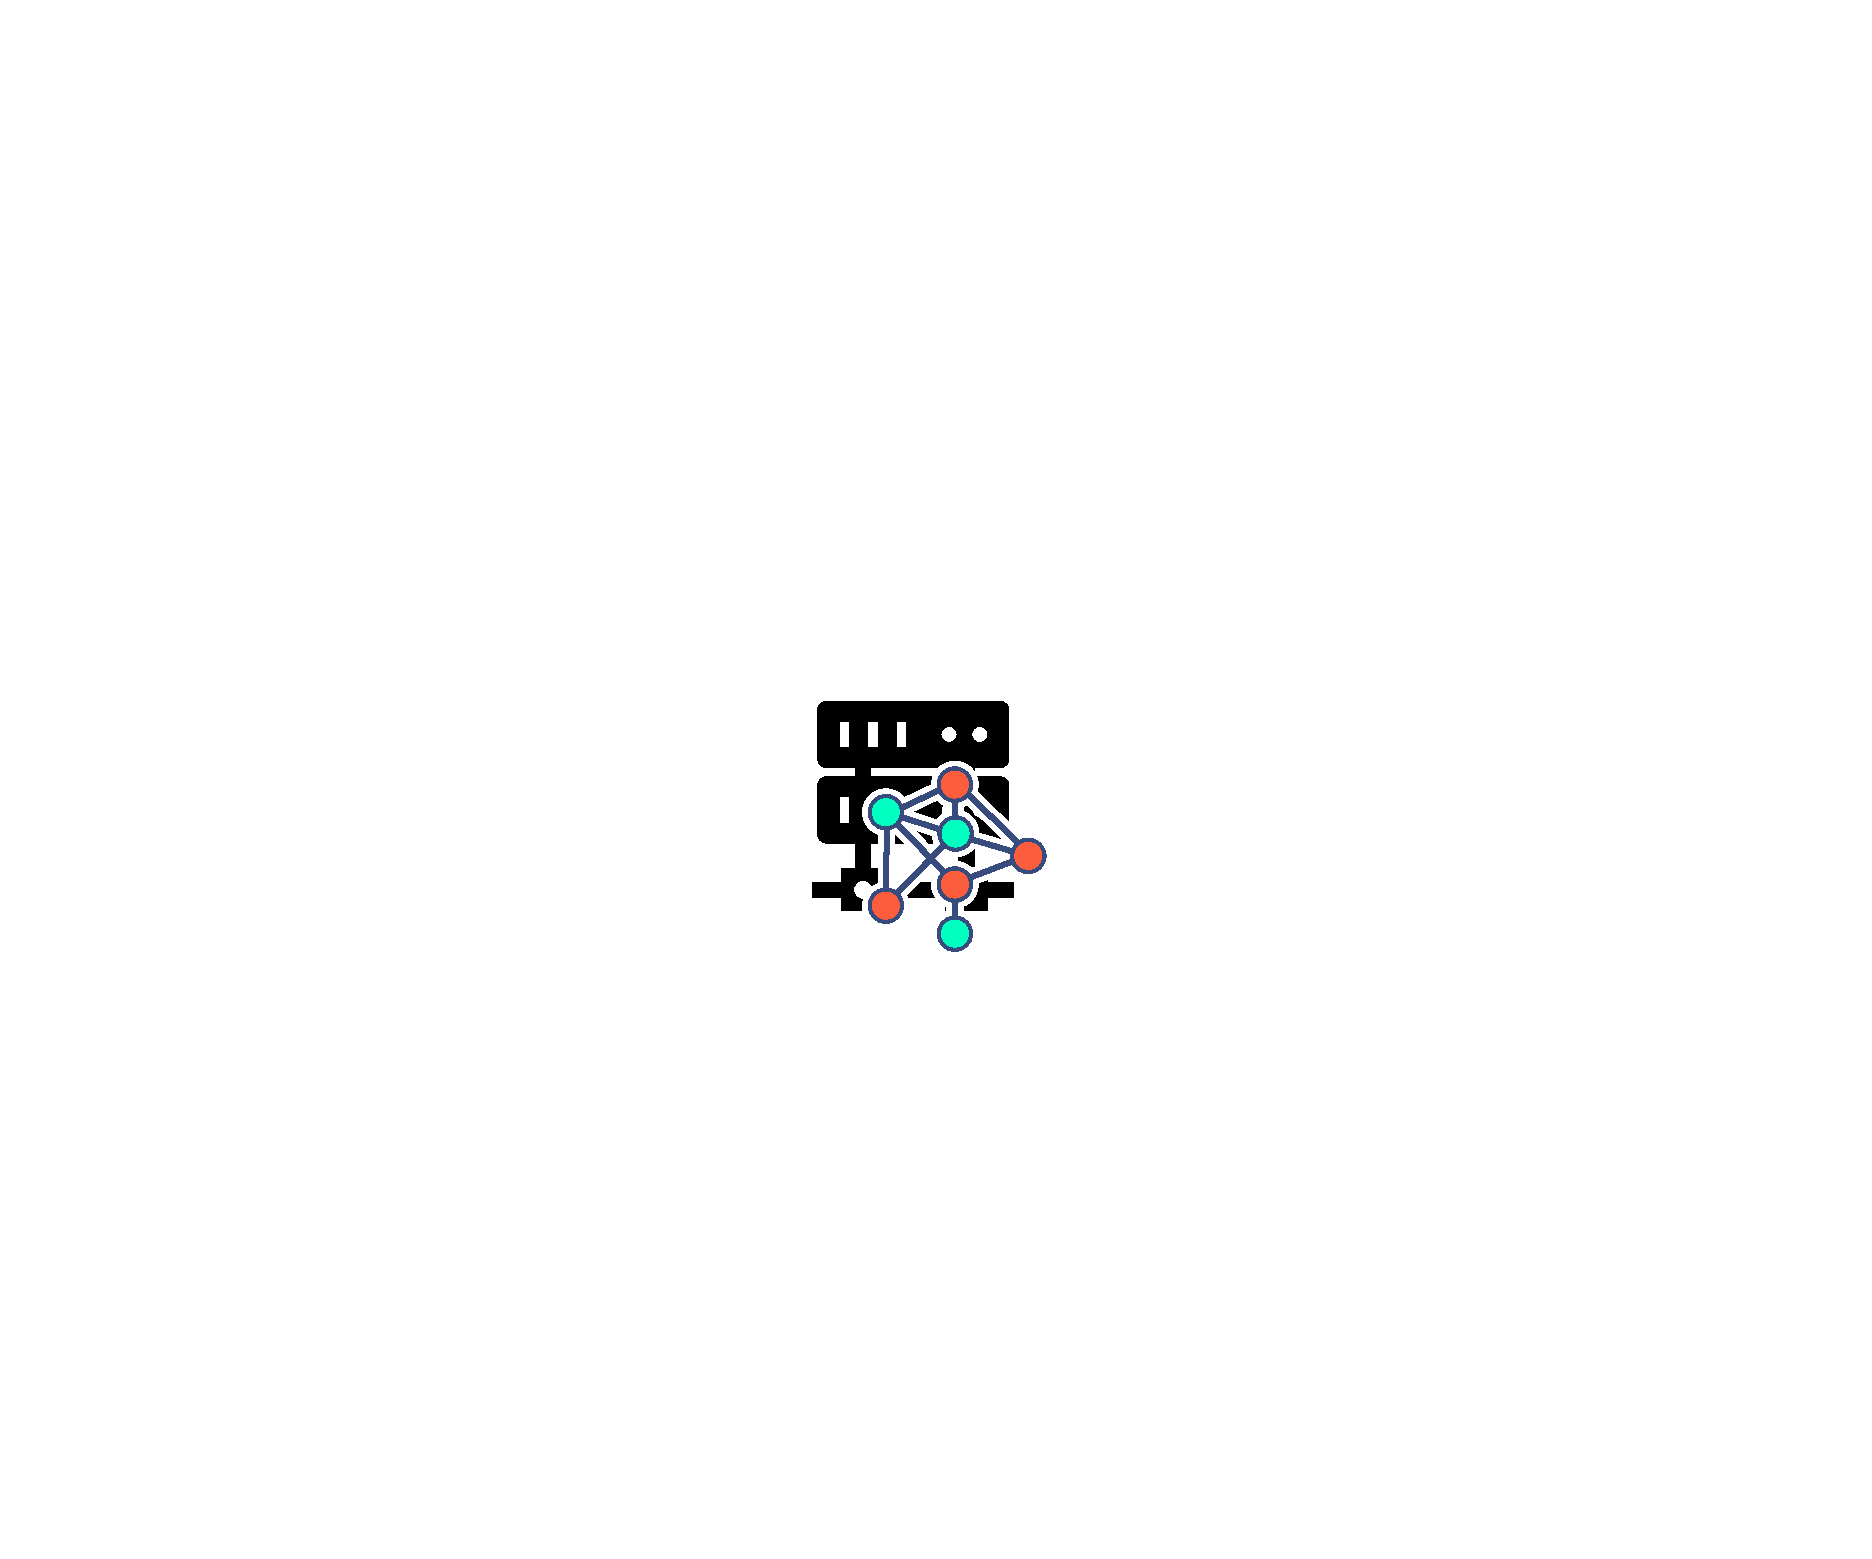
\includegraphics[width=\linewidth]{images/federated_learning_only_server.pdf} }%
    \only<2,3,4>{    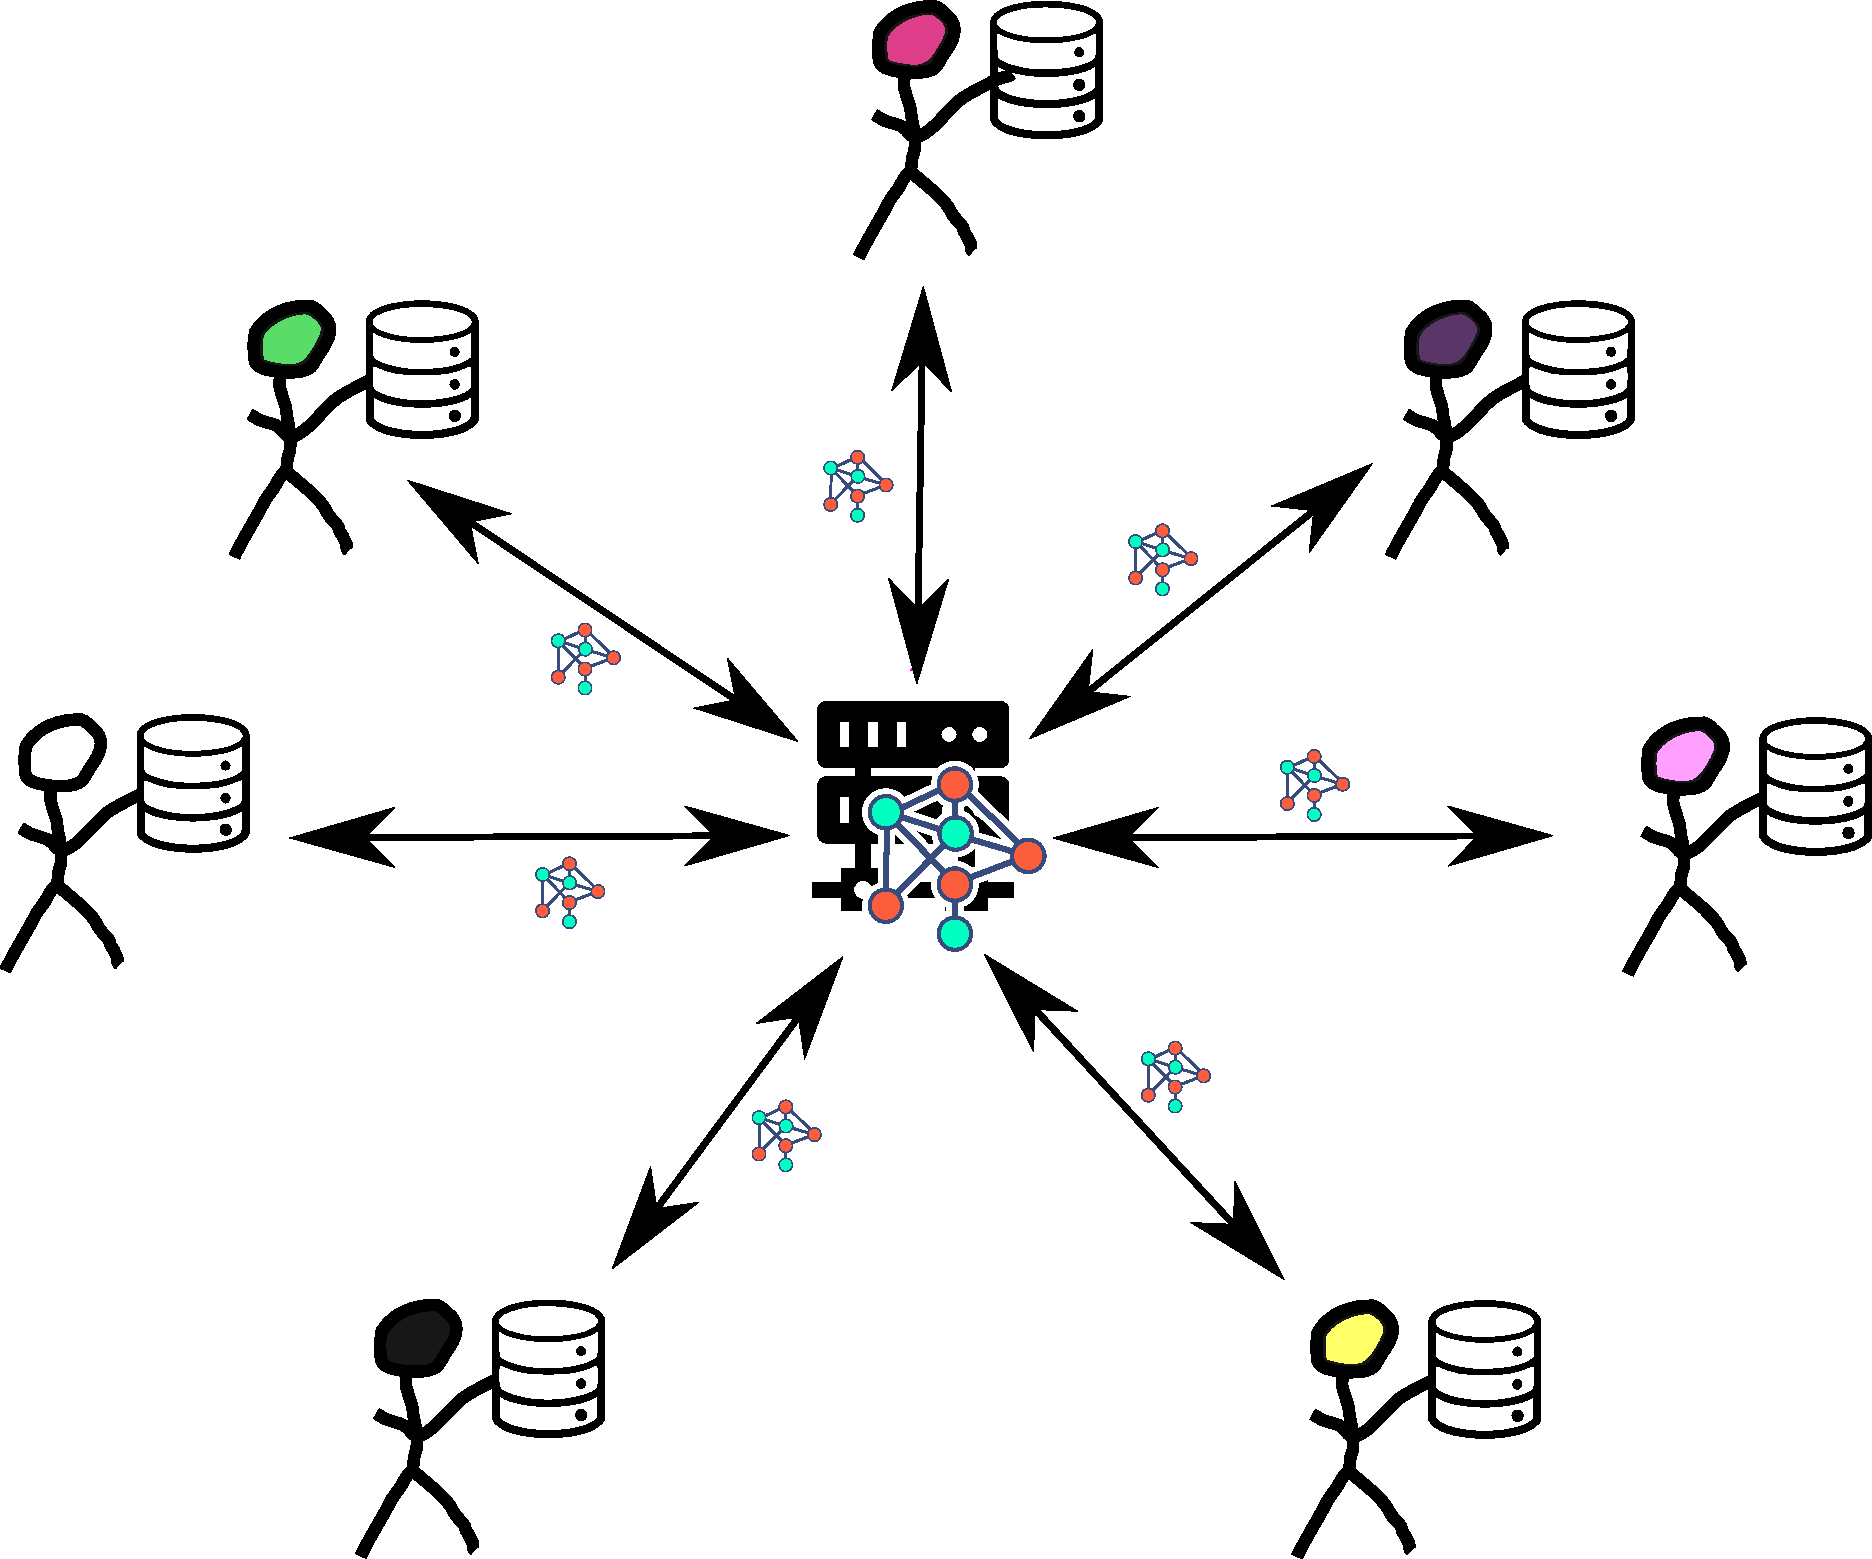
\includegraphics[width=\linewidth]{images/federated_learning.pdf} }
    \end{center}
    
  \end{minipage}~~~~~~%
  \begin{minipage}{0.5\linewidth}

\only<3,4>{
    \begin{center}
      Optimisation collaborative
      \begin{align*}
        \min_{x \in \mathbb{R}^d} 
        \frac{1}{N} \sum_{c=1}^N f_c(x)
        ~~,
        \quad 
        f_c(x)
        = \mathbb{E}_Z[ F_c(x; Z) ]
      \end{align*}
      % $\rightarrow$ avec une seule \emph{solution globale}
    \end{center}
    }
      
  \end{minipage}

\vspace{0.5em}

\only<4>{
  \begin{center}
      \textbf{\textcolor{purple}{Difficultés centrales}} : hétérogénéité des données et des moyens de calcul 

      \vspace{-0.5em}
      
      + communication lente et difficile à établir
  \end{center}
}

\end{frame}




\begin{frame}[t]{Optimisation fédérée ~~~ \raisebox{0.2em}{\textcolor{black}{\normalsize $x^\star \in \arg\min_{x \in \mathbb{R}^d} 
    \frac{1}{N} \sum_{c=1}^N \mathbb{E}_Z[ F_c(x; Z) ]$}} ~~}  
    
    \vspace{-1em}

  \begin{minipage}{0.5\linewidth}
  Federated Averaging\footfullcite{mcmahan2017communicationoral} (FedAvg)

\vspace{0.5em}
    

  \footnotesize
  À chaque itération globale :

    \begin{itemize}[leftmargin=*,itemsep=0em]
  \footnotesize
    \item Pour $c=1$ à $N$ en parallèle

\vspace{-0.2em}
    
    
\begin{itemize}[leftmargin=*,itemsep=0em]
\item Recevoir $x^{(t)}$, initialiser $x^{(t,0)}_c = x^{(t)}$
    
        \item Pour $h=0$ à $H-1$
    \end{itemize}

\vspace{-0.6em}
\begin{center}
            \hspace{-1em}$x^{(t,h+1)}_c = x^{(t,h)}_c - \gamma \nabla F_c( x^{(t,h)}_c ; Z_c^{(t,h+1)})$
        \end{center}
      
  \item Agrégation des modèles
        
        
\vspace{-0.6em}
\begin{center}
            \hspace{-1em}$x^{(t+1)} = \frac{1}{N} \sum_{c=1}^N x_c^{(t,H)}$
        \end{center}
      
    \end{itemize}
      
  \end{minipage}~%
  \begin{minipage}{0.48\linewidth}
  \pause
       \begin{center}
    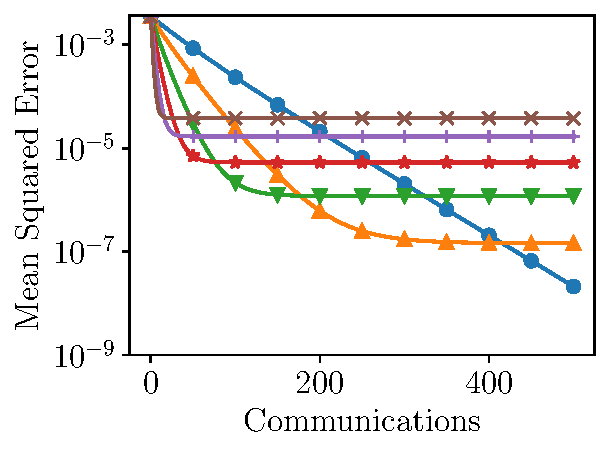
\includegraphics[width=0.75\linewidth]{images/local_training_heterogeneous.pdf}%
    \raisebox{2.5em}{ 
\includegraphics[width=0.25\linewidth]{images/legend.pdf} }
  \end{center}
  
    \vspace{-0.5em}

  ~~~~Plus d'itérations locales

    \vspace{0.5em}
    
    ~~~~~{\large \textcolor{green} \cmark}\, convergence plus rapide
    
    ~~~~~{\large \textcolor{red} \xmark}~ biais plus grand

  \end{minipage}

  \vspace{1.5em}


\end{frame}


\begin{frame}[t]{FedAvg avec gradients stochastiques converge !\footfullcite{mangold2025refined}}

{\small Si $f_c$ trois fois dérivable, $\mu$-fortement convexe, $\nabla f_c$ est $L$-Lipschitz, et $\gamma \le 1/L$}
\begin{itemize}[leftmargin=*]
    \item FedAvg converge en Wasserstein vers une distribution $\pi^{(\gamma, H)}$
    \only<2>{
    \begin{itemize}
        \item et si $x^{(t)} \sim \psi_{x^{(t)}}$,
    \begin{align*}
        \mathcal{W}_2(\psi_{x^{(t)}}; \pi^{(\gamma, H)})
        \le
        (1 - \gamma \mu)^{H t} \mathcal{W}_2(\psi_{x^{(0)}}; \pi^{(\gamma, H)})
    \end{align*}
    \item où $\mathcal{W}_2$ est la distance de Wasserstein d'ordre 2
    \end{itemize}
    }

\pause

\pause


    \item Biais  de FedAvg (pour $\gamma, H$ petits) 
    \only<3,4>{
    \begin{align*}
    \int x \pi^{(\gamma, H)}(\mathrm{d} x)
    &  = x^\star +
    \tikz[remember picture,baseline=(heterbias.base)] \node[blueblock] (heterbias) at (0,0) {
    \textnormal{$\displaystyle \frac{\gamma (H-1)}{2N}
    \sum_{c=1}^N \nabla^2 f(x^\star)^{-1}
    \big( \nabla^2 f_c(x^\star) - \nabla^2 f(x^\star) \big)
    \nabla f_c(x^\star)$}
    };
    \\ 
    &  \qquad
    -  \tikz[remember picture,baseline=(stobias.base)] \node[pinkblock] (stobias) at (0,0) {
    \textnormal{$\displaystyle
    \frac{\gamma}{2 N} \nabla^2 f(x^\star)^{-1}
    \nabla^3 f(x^\star) A^{-1} C(x^\star)
    $}};
    + O(\gamma^2 H^2)
    \end{align*}
    }
\pause

\only<3,4>{
\begin{tikzpicture}[overlay,remember picture]
    \node[blueblock] (heterbiaslegend) at (3,6) {\shortstack{\underline{Biais d'hétérogénéité} \\[0.5em]
     Disparaît quand $\nabla^2 f_c(x^\star) = \nabla^2 f(x^\star)$ \\
    \quad ou quand $\nabla f_c(x^\star) = \nabla f(x^\star)$
    }};
    \draw[color=amethyst] (heterbias) -- (heterbiaslegend);
    
    \node[pinkblock] (stobiaslegend) at (10.5,6) {\shortstack{\underline{Biais de stochasticité} \\[0.5em]
    $A$ est un opérateur linéaire \\
    $C(x^\star)$ est la covariance de $\nabla f$ en $x^\star$
    }};
    \draw[color=amaranth] (stobias) -- (stobiaslegend);
\end{tikzpicture}

\vspace{-4em}
}

\pause

    \item Variance  de FedAvg (pour $\gamma, H$ petits) 
    \only<5,6>{
    \begin{align*}
    \int (x - x^\star)(x - x^\star)^\top \pi^{(\gamma, H)}(\mathrm{d} x)
    &  =
    \tikz[remember picture,baseline=(variance.base)] \node[pinkblock] (variance) at (0,0) {
    \textnormal{$\displaystyle \frac{\gamma}{N} C(x^\star) $}}; + O(\gamma^2 H^2)
    \end{align*}
    }
\pause

\only<5,6>{
\begin{tikzpicture}[overlay,remember picture]
    \node[pinkblock] (variancelegend) at (5,4) {\shortstack{\underline{Linear speed-up !} \\[0.5em]
    variance decreases in $1/N$ \\
    variance scales in $\gamma$
    }};
    \draw[color=amethyst] (variance) -- (variancelegend);
\end{tikzpicture}

\vspace{-4em}
}

\end{itemize}

\end{frame}


\begin{frame}[t]{Scaffold ~~~ \raisebox{0.2em}{\textcolor{black}{\normalsize $x^\star \in \arg\min_{x \in \mathbb{R}^d} 
    \frac{1}{N} \sum_{c=1}^N \mathbb{E}_Z[ F_c(x; Z) ]$}} ~~}  
    
    \vspace{-1em}

  \begin{minipage}{0.5\linewidth}

  \footnotesize
  À chaque itération globale :

    \begin{itemize}[leftmargin=*,itemsep=0em]
  \footnotesize
    \item Pour $c=1$ à $N$ en parallèle

\vspace{-0.2em}
    
    
\begin{itemize}[leftmargin=*,itemsep=0em]
\item Recevoir $x^{(t)}$, initialiser $x^{(t,0)}_c = x^{(t)}$
    
        \item Pour $h=0$ à $H-1$
    \end{itemize}

\vspace{-0.6em}
\begin{center}
            \hspace{-1em}$x^{(t,h+1)}_c = x^{(t,h)}_c - \gamma \big( \nabla F_c( x^{(t,h)}_c ; Z_c^{(t,h+1)}) + \xi_c^{(t)} \big)$
        \end{center}
      
  \item Agrégation des modèles
        
        
\vspace{-0.6em}
\begin{center}
            \hspace{-1em}$x^{(t+1)} = \frac{1}{N} \sum_{c=1}^N x_c^{(t,H)}$
          \end{center}
\begin{center}
            \hspace{-1em}$\xi_c^{(t+1)} = \xi_c^{(t)} + \frac{1}{\gamma H} (\theta_c^{t,H} - \theta^{(t+1)} )$
          \end{center}

          
      
    \end{itemize}
      
  \end{minipage}~%
  \begin{minipage}{0.48\linewidth}
  \pause
       \begin{center}
    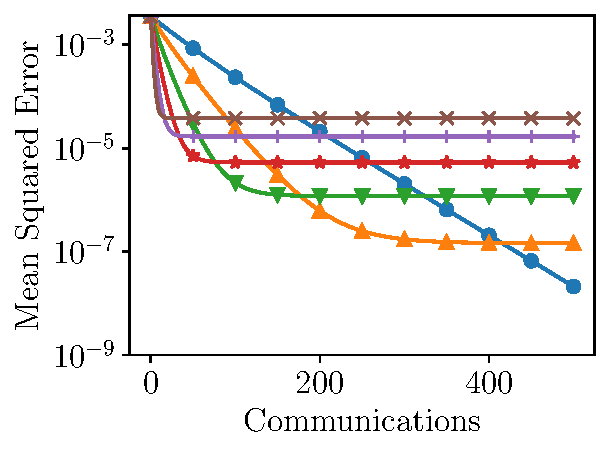
\includegraphics[width=0.75\linewidth]{images/local_training_heterogeneous.pdf}%
    \raisebox{2.5em}{ 
\includegraphics[width=0.25\linewidth]{images/legend.pdf} }
  \end{center}
  
    \vspace{-0.5em}

  $\rightarrow$ No more heterogeneity bias!

  \end{minipage}

  \vspace{1.5em}


\end{frame}




\begin{frame}[t]{Scaffold also converges !\footfullcite{mangold2025refined}}

{\small Si $f_c$ trois fois dérivable, $\mu$-fortement convexe, $\nabla f_c$ est $L$-Lipschitz, et $\gamma \le 1/L$}
\begin{itemize}[leftmargin=*]
    \item Scaffold converges if $\gamma H L \le 1$ en Wasserstein vers une distribution $\pi^{(\gamma, H)}$
    \only<2>{
    \begin{itemize}
        \item et si $x^{(t)} \sim \psi_{x^{(t)}}$,
    \begin{align*}
        \mathcal{W}_2(\psi_{x^{(t)}}; \pi^{(\gamma, H)})
        \le
        (1 - \gamma \mu)^{H t} \mathcal{W}_2(\psi_{x^{(0)}}; \pi^{(\gamma, H)})
    \end{align*}
    \item où $\mathcal{W}_2$ est la distance de Wasserstein d'ordre 2
    \end{itemize}
    }

\pause

\pause


    \item Biais  de Scaffold (pour $\gamma, H$ petits) 
    \only<3,4>{
    \begin{align*}
    \int x \pi^{(\gamma, H)}(\mathrm{d} x)
    &  = x^\star
    -  \tikz[remember picture,baseline=(stobias.base)] \node[pinkblock] (stobias) at (0,0) {
    \textnormal{$\displaystyle
    \frac{\gamma}{2 N} \nabla^2 f(x^\star)^{-1}
    \nabla^3 f(x^\star) A^{-1} C(x^\star)
    $}};
    + O(\gamma^2 H^2)
    \end{align*}
    }
\pause

\only<3,4>{
\begin{tikzpicture}[overlay,remember picture]    
    \node[pinkblock] (stobiaslegend) at (10.5,6) {\shortstack{\underline{Biais de stochasticité} \\[0.5em]
    $A$ est un opérateur linéaire \\
    $C(x^\star)$ est la covariance de $\nabla f$ en $x^\star$
    }};
    \draw[color=amaranth] (stobias) -- (stobiaslegend);
\end{tikzpicture}

\vspace{-4em}
}

\pause

    \item Variance  de FedAvg (pour $\gamma, H$ petits) 
    \only<5,6>{
    \begin{align*}
    \int (x - x^\star)(x - x^\star)^\top \pi^{(\gamma, H)}(\mathrm{d} x)
    &  =
    \tikz[remember picture,baseline=(variance.base)] \node[pinkblock] (variance) at (0,0) {
    \textnormal{$\displaystyle \frac{\gamma}{N} C(x^\star) $}}; + O(\gamma^2 H^2)
    \end{align*}
    }
\pause

\only<5,6>{
\begin{tikzpicture}[overlay,remember picture]
    \node[pinkblock] (variancelegend) at (5,4) {\shortstack{\underline{Linear speed-up !} \\[0.5em]
    variance decreases in $1/N$ \\
    variance scales in $\gamma$
    }};
    \draw[color=amethyst] (variance) -- (variancelegend);
\end{tikzpicture}

\vspace{-4em}
}

\end{itemize}

\end{frame}

\begin{frame}{New Convergence Rate for Scaffold}


  
\end{frame}

\begin{frame}{Linear Speed-Up!}


  
\end{frame}

\begin{frame}{Numerical Illustrations}


  
\end{frame}

\begin{frame}{Conclusion}


  
\end{frame}


\end{document}
%%% Local Variables:
%%% mode: latex
%%% TeX-master: t
%%% End:
